\begin{frame}[fragile]
  \frametitle{Пример}
\begin{center}
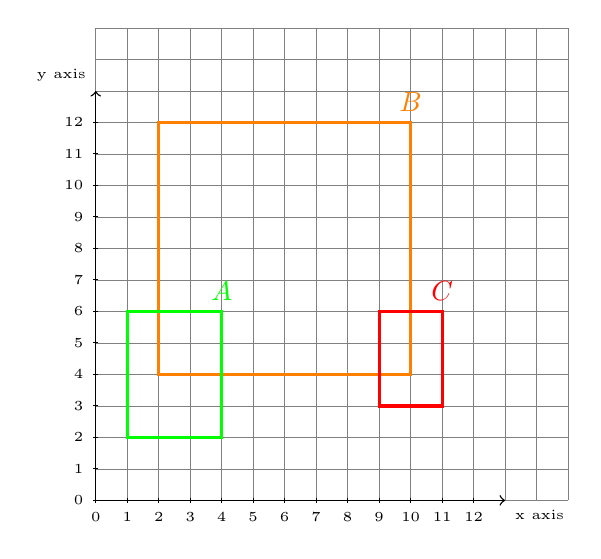
\begin{tikzpicture}
\draw[step=0.4cm,gray,very thin] (0.0,0.0) grid (6,6);
\draw[orange, very thick] (0.8,1.6) rectangle (4.0,4.8) node[anchor=south] {$B$};
\draw[green, very thick] (0.4,0.8) rectangle (1.6,2.4) node[anchor=south] {$A$};
\draw[red, very thick] (3.6,1.2) rectangle (4.4,2.4) node[anchor=south] {$C$};
\foreach \x in {0,1,2,3,4,5,6,7,8,9,10,11,12}
    \draw (\x * 0.4 cm,1pt) -- (\x * 0.4 cm,-1pt) node[anchor=north] {\tiny $\x$};
\foreach \y in {0,1,2,3,4,5,6,7,8,9,10,11,12}
    \draw (1pt,\y * 0.4 cm) -- (-1pt,\y * 0.4 cm) node[anchor=east] {\tiny $\y$};

\draw[->, line width=0.5pt] (0,0) -- (5.2,0) node[anchor=north west] {\tiny x axis};
\draw[->, line width=0.5pt] (0,0) -- (0,5.2) node[anchor=south east] {\tiny y axis};
\end{tikzpicture}
\end{center}
\end{frame}

\definecolor{activecolor}{rgb}{1.0, 1.0, 1.0}
\definecolor{deadcolor}{rgb}{0.4, 0.4, 0.4}


\begin{frame}[fragile]
\frametitle{test\_rectangle.cpp}
\begin{minipage}[t]{0.48\linewidth}
\begin{lstlisting}
#include "doctest.h"

TEST_CASE("Create rectangle") {
    Rectangle a(0, 0, 10, 12);
}
\end{lstlisting}
\end{minipage}\hfill
\begin{minipage}[t]{0.28\linewidth}
  \small
  \begin{enumerate} 
    \item \textcolor{activecolor}{Write a test}
    \item \textcolor{deadcolor}{Make it compile}
    \item \textcolor{deadcolor}{Run it (fails)}
    \item \textcolor{deadcolor}{Make it pass}
    \item \textcolor{deadcolor}{Improve quality}
  \end{enumerate} 
\end{minipage}
\end{frame}



\begin{frame}[fragile]
\frametitle{test\_rectangle.cpp}
\begin{minipage}[t]{0.48\linewidth}
\begin{lstlisting}
#include "doctest.h"

TEST_CASE("Create rectangle") {
    Rectangle a(0, 0, 10, 12);
}
\end{lstlisting}
\end{minipage}\hfill
\begin{minipage}[t]{0.28\linewidth}
  \small
  \begin{enumerate} 
    \item \textcolor{deadcolor}{Write a test}
    \item \textcolor{activecolor}{Make it compile}
    \item \textcolor{deadcolor}{Run it (fails)}
    \item \textcolor{deadcolor}{Make it pass}
    \item \textcolor{deadcolor}{Improve quality}
  \end{enumerate} 
\end{minipage}
\end{frame}


\begin{frame}[fragile]
\frametitle{rectangle.h}
\begin{minipage}[t]{0.48\linewidth}
\begin{lstlisting}
struct Rectangle {
    Rectangle(int x, int y, int width, int height);
    int x, y;
    int width, height;
};
\end{lstlisting}
\end{minipage}\hfill
\begin{minipage}[t]{0.28\linewidth}
  \small
  \begin{enumerate} 
    \item \textcolor{deadcolor}{Write a test}
    \item \textcolor{activecolor}{Make it compile}
    \item \textcolor{deadcolor}{Run it (fails)}
    \item \textcolor{deadcolor}{Make it pass}
    \item \textcolor{deadcolor}{Improve quality}
  \end{enumerate} 
\end{minipage}
\end{frame}


\begin{frame}[fragile]
\frametitle{test\_rectangle.cpp}
\begin{minipage}[t]{0.48\linewidth}
\begin{lstlisting}
#include "doctest.h"
#include "rectangle.h"

TEST_CASE("Create rectangle") {
    Rectangle a(0, 0, 10, 12);
}
\end{lstlisting}
\end{minipage}\hfill
\begin{minipage}[t]{0.28\linewidth}
  \small
  \begin{enumerate} 
    \item \textcolor{deadcolor}{Write a test}
    \item \textcolor{activecolor}{Make it compile}
    \item \textcolor{deadcolor}{Run it (fails)}
    \item \textcolor{deadcolor}{Make it pass}
    \item \textcolor{deadcolor}{Improve quality}
  \end{enumerate} 
\end{minipage}
\end{frame}


\begin{frame}[fragile]
\frametitle{rectangle.cpp}
\begin{minipage}[t]{0.48\linewidth}
\begin{lstlisting}
#include "rectangle.h"

Rectangle::Rectangle(int x, int y, 
                     int width, int height){
}
\end{lstlisting}
\end{minipage}\hfill
\begin{minipage}[t]{0.28\linewidth}
  \small
  \begin{enumerate} 
    \item \textcolor{deadcolor}{Write a test}
    \item \textcolor{activecolor}{Make it compile}
    \item \textcolor{deadcolor}{Run it (fails)}
    \item \textcolor{deadcolor}{Make it pass}
    \item \textcolor{deadcolor}{Improve quality}
  \end{enumerate} 
\end{minipage}
\end{frame}

\begin{frame}[fragile]
\frametitle{Run doctest}
\begin{minipage}[t]{0.48\linewidth}
test cases: 1 | 1 passed | 0 failed\\
assertions: 0 | 0 passed | 0 failed\\
\end{minipage}\hfill
\begin{minipage}[t]{0.28\linewidth}
  \small
  \begin{enumerate} 
    \item \textcolor{deadcolor}{Write a test}
    \item \textcolor{deadcolor}{Make it compile}
    \item \textcolor{activecolor}{Run it (fails)}
    \item \textcolor{deadcolor}{Make it pass}
    \item \textcolor{deadcolor}{Improve quality}
  \end{enumerate} 
\end{minipage}
\end{frame}


\begin{frame}[fragile]
\frametitle{test\_rectangle.cpp}
\begin{minipage}[t]{0.48\linewidth}
\begin{lstlisting}
#include "doctest.h"
#include "rectangle.h"

TEST_CASE("Create rectangle") {
    Rectangle a(0, 0, 10, 12);
    REQUIRE(a.x == 0);
    REQUIRE(a.y == 0);
    REQUIRE(a.width == 10);
    REQUIRE(a.height == 12);
}
\end{lstlisting}
\end{minipage}\hfill
\begin{minipage}[t]{0.28\linewidth}
  \small
  \begin{enumerate} 
    \item \textcolor{activecolor}{Write a test}
    \item \textcolor{deadcolor}{Make it compile}
    \item \textcolor{deadcolor}{Run it (fails)}
    \item \textcolor{deadcolor}{Make it pass}
    \item \textcolor{deadcolor}{Improve quality}
  \end{enumerate} 
\end{minipage}
\end{frame}


\begin{frame}[fragile]
\frametitle{test\_rectangle.cpp}
\begin{minipage}[t]{0.48\linewidth}
\begin{lstlisting}
#include "doctest.h"
#include "rectangle.h"

TEST_CASE("Create rectangle") {
    Rectangle a(0, 0, 10, 12);
    REQUIRE(a.x == 0);
    REQUIRE(a.y == 0);
    REQUIRE(a.width == 10);
    REQUIRE(a.height == 12);
}
\end{lstlisting}
\end{minipage}\hfill
\begin{minipage}[t]{0.28\linewidth}
  \small
  \begin{enumerate} 
    \item \textcolor{deadcolor}{Write a test}
    \item \textcolor{activecolor}{Make it compile}
    \item \textcolor{deadcolor}{Run it (fails)}
    \item \textcolor{deadcolor}{Make it pass}
    \item \textcolor{deadcolor}{Improve quality}
  \end{enumerate} 
\end{minipage}
\end{frame}


\begin{frame}[fragile]
\frametitle{Run doctest}
\begin{minipage}[t]{0.48\linewidth}
test cases: 1 | 0 passed | 1 failed\\
assertions: 4 | 0 passed | 4 failed\\
\end{minipage}\hfill
\begin{minipage}[t]{0.28\linewidth}
  \small
  \begin{enumerate} 
    \item \textcolor{deadcolor}{Write a test}
    \item \textcolor{deadcolor}{Make it compile}
    \item \textcolor{activecolor}{Run it (fails)}
    \item \textcolor{deadcolor}{Make it pass}
    \item \textcolor{deadcolor}{Improve quality}
  \end{enumerate} 
\end{minipage}
\end{frame}



\begin{frame}[fragile]
\frametitle{rectangle.cpp}
\begin{minipage}[t]{0.48\linewidth}
\begin{lstlisting}
#include "rectangle.h"

Rectangle::Rectangle(int x, int y, 
                     int width, int height){
}
\end{lstlisting}
\end{minipage}\hfill
\begin{minipage}[t]{0.28\linewidth}
  \small
  \begin{enumerate} 
    \item \textcolor{deadcolor}{Write a test}
    \item \textcolor{deadcolor}{Make it compile}
    \item \textcolor{deadcolor}{Run it (fails)}
    \item \textcolor{activecolor}{Make it pass}
    \item \textcolor{deadcolor}{Improve quality}
  \end{enumerate} 
\end{minipage}
\end{frame}

\begin{frame}[fragile]
\frametitle{rectangle.cpp}
\begin{minipage}[t]{0.48\linewidth}
\begin{lstlisting}
#include "rectangle.h"

Rectangle::Rectangle(int x, int y, 
                     int width, int height)
    : x(x), y(y), width(width), height(height) {}

\end{lstlisting}
\end{minipage}\hfill
\begin{minipage}[t]{0.28\linewidth}
  \small
  \begin{enumerate} 
    \item \textcolor{deadcolor}{Write a test}
    \item \textcolor{deadcolor}{Make it compile}
    \item \textcolor{deadcolor}{Run it (fails)}
    \item \textcolor{activecolor}{Make it pass}
    \item \textcolor{deadcolor}{Improve quality}
  \end{enumerate} 
\end{minipage}
\end{frame}

\begin{frame}[fragile]
\frametitle{Run doctest}
\begin{minipage}[t]{0.48\linewidth}
test cases: 1 | 1 passed | 0 failed\\
assertions: 4 | 4 passed | 0 failed\\
\end{minipage}\hfill
\begin{minipage}[t]{0.28\linewidth}
  \small
  \begin{enumerate} 
    \item \textcolor{deadcolor}{Write a test}
    \item \textcolor{deadcolor}{Make it compile}
    \item \textcolor{deadcolor}{Run it (fails)}
    \item \textcolor{activecolor}{Make it pass}
    \item \textcolor{deadcolor}{Improve quality}
  \end{enumerate} 
\end{minipage}
\end{frame}


\begin{frame}[fragile]
\frametitle{rectangle.cpp}
\begin{minipage}[t]{0.48\linewidth}
\begin{lstlisting}
#include "rectangle.h"

Rectangle::Rectangle(int x, int y, 
                     int width, int height)
    : x(x), y(y), width(width), height(height) {}

\end{lstlisting}
\end{minipage}\hfill
\begin{minipage}[t]{0.28\linewidth}
  \small
  \begin{enumerate} 
    \item \textcolor{deadcolor}{Write a test}
    \item \textcolor{deadcolor}{Make it compile}
    \item \textcolor{deadcolor}{Run it (fails)}
    \item \textcolor{deadcolor}{Make it pass}
    \item \textcolor{activecolor}{Improve quality}
  \end{enumerate} 
\end{minipage}
\end{frame}



\begin{frame}[fragile]
\frametitle{test\_rectangle.cpp}
\begin{minipage}[t]{0.48\linewidth}
\begin{lstlisting}
#include "doctest.h"
#include "rectangle.h"

TEST_CASE("Create rectangle") {
    Rectangle a(0, 0, 10, 12);
    REQUIRE(a.x == 0);
    REQUIRE(a.y == 0);
    REQUIRE(a.width == 10);
    REQUIRE(a.height == 12);
}
\end{lstlisting}
\end{minipage}\hfill
\begin{minipage}[t]{0.28\linewidth}
  \small
  \begin{enumerate} 
    \item \textcolor{deadcolor}{Write a test}
    \item \textcolor{deadcolor}{Make it compile}
    \item \textcolor{deadcolor}{Run it (fails)}
    \item \textcolor{deadcolor}{Make it pass}
    \item \textcolor{activecolor}{Improve quality}
  \end{enumerate} 
\end{minipage}
\end{frame}


\begin{frame}[fragile]
\frametitle{test\_rectangle.cpp}
\begin{minipage}[t]{0.48\linewidth}
\begin{lstlisting}
....

TEST_CASE("Test overlapping rectangles") {
    Rectangle a(0, 0, 10, 12);
    Rectangle b(1, 2, 3, 4);
    bool overlap = a.overlap(b);
    REQUIRE(overlap == true);
}
\end{lstlisting}
\end{minipage}\hfill
\begin{minipage}[t]{0.28\linewidth}
  \small
  \begin{enumerate} 
    \item \textcolor{activecolor}{Write a test}
    \item \textcolor{deadcolor}{Make it compile}
    \item \textcolor{deadcolor}{Run it (fails)}
    \item \textcolor{deadcolor}{Make it pass}
    \item \textcolor{deadcolor}{Improve quality}
  \end{enumerate} 
\end{minipage}
\end{frame}

\begin{frame}[fragile]
\frametitle{test\_rectangle.cpp}
\begin{minipage}[t]{0.48\linewidth}
\begin{lstlisting}
....

TEST_CASE("Test overlapping rectangles") {
    Rectangle a(0, 0, 10, 12);
    Rectangle b(1, 2, 3, 4);
    bool overlap = a.overlap(b);
    REQUIRE(overlap == true);
}
\end{lstlisting}
\end{minipage}\hfill
\begin{minipage}[t]{0.28\linewidth}
  \small
  \begin{enumerate} 
    \item \textcolor{deadcolor}{Write a test}
    \item \textcolor{activecolor}{Make it compile}
    \item \textcolor{deadcolor}{Run it (fails)}
    \item \textcolor{deadcolor}{Make it pass}
    \item \textcolor{deadcolor}{Improve quality}
  \end{enumerate} 
\end{minipage}
\end{frame}

\begin{frame}[fragile]
\frametitle{rectangle.h}
\begin{minipage}[t]{0.48\linewidth}
\begin{lstlisting}
struct Rectangle {
    Rectangle(int x, int y, int width, int height);
    int x, y;
    int width, height;
};
\end{lstlisting}
\end{minipage}\hfill
\begin{minipage}[t]{0.28\linewidth}
  \small
  \begin{enumerate} 
    \item \textcolor{deadcolor}{Write a test}
    \item \textcolor{activecolor}{Make it compile}
    \item \textcolor{deadcolor}{Run it (fails)}
    \item \textcolor{deadcolor}{Make it pass}
    \item \textcolor{deadcolor}{Improve quality}
  \end{enumerate} 
\end{minipage}
\end{frame}

\begin{frame}[fragile]
\frametitle{rectangle.h}
\begin{minipage}[t]{0.48\linewidth}
\begin{lstlisting}
struct Rectangle {
    Rectangle(int x, int y, int width, int height);
    int x, y;
    int width, height;
    bool overlap(const Rectangle & other) const;
};
\end{lstlisting}
\end{minipage}\hfill
\begin{minipage}[t]{0.28\linewidth}
  \small
  \begin{enumerate} 
    \item \textcolor{deadcolor}{Write a test}
    \item \textcolor{activecolor}{Make it compile}
    \item \textcolor{deadcolor}{Run it (fails)}
    \item \textcolor{deadcolor}{Make it pass}
    \item \textcolor{deadcolor}{Improve quality}
  \end{enumerate} 
\end{minipage}
\end{frame}


\begin{frame}[fragile]
\frametitle{rectangle.cpp}
\begin{minipage}[t]{0.48\linewidth}
\begin{lstlisting}
#include "rectangle.h"

Rectangle::Rectangle(int x, int y, 
                     int width, int height)
    : x(x), y(y), width(width), height(height) {}

\end{lstlisting}
\end{minipage}\hfill
\begin{minipage}[t]{0.28\linewidth}
  \small
  \begin{enumerate} 
    \item \textcolor{deadcolor}{Write a test}
    \item \textcolor{activecolor}{Make it compile}
    \item \textcolor{deadcolor}{Run it (fails)}
    \item \textcolor{deadcolor}{Make it pass}
    \item \textcolor{deadcolor}{Improve quality}
  \end{enumerate} 
\end{minipage}
\end{frame}


\begin{frame}[fragile]
\frametitle{rectangle.cpp}
\begin{minipage}[t]{0.48\linewidth}
\begin{lstlisting}
#include "rectangle.h"

Rectangle::Rectangle(int x, int y, 
                     int width, int height)
    : x(x), y(y), width(width), height(height) {}

bool 
Rectangle::overlap(const Rectangle &other)const{
    return false;
}
\end{lstlisting}
\end{minipage}\hfill
\begin{minipage}[t]{0.28\linewidth}
  \small
  \begin{enumerate} 
    \item \textcolor{deadcolor}{Write a test}
    \item \textcolor{activecolor}{Make it compile}
    \item \textcolor{deadcolor}{Run it (fails)}
    \item \textcolor{deadcolor}{Make it pass}
    \item \textcolor{deadcolor}{Improve quality}
  \end{enumerate} 
\end{minipage}
\end{frame}

\begin{frame}[fragile]
\frametitle{rectangle.cpp}
\begin{minipage}[t]{0.48\linewidth}
\begin{lstlisting}
...

bool 
Rectangle::overlap(const Rectangle &other)const{
    return false;
}
\end{lstlisting}
\end{minipage}\hfill
\begin{minipage}[t]{0.28\linewidth}
  \small
  \begin{enumerate} 
    \item \textcolor{deadcolor}{Write a test}
    \item \textcolor{activecolor}{Make it compile}
    \item \textcolor{deadcolor}{Run it (fails)}
    \item \textcolor{deadcolor}{Make it pass}
    \item \textcolor{deadcolor}{Improve quality}
  \end{enumerate} 
\end{minipage}
\end{frame}



\begin{frame}[fragile]
\frametitle{Run doctest}
\begin{minipage}[t]{0.48\linewidth}
test cases: 2 | 1 passed | 1 failed\\
assertions: 5 | 4 passed | 1 failed\\
\end{minipage}\hfill
\begin{minipage}[t]{0.28\linewidth}
  \small
  \begin{enumerate} 
    \item \textcolor{deadcolor}{Write a test}
    \item \textcolor{deadcolor}{Make it compile}
    \item \textcolor{activecolor}{Run it (fails)}
    \item \textcolor{deadcolor}{Make it pass}
    \item \textcolor{deadcolor}{Improve quality}
  \end{enumerate} 
\end{minipage}
\end{frame}


\begin{frame}[fragile]
\frametitle{rectangle.cpp}
\begin{minipage}[t]{0.48\linewidth}
\begin{lstlisting}
...

bool 
Rectangle::overlap(const Rectangle &other)const{
    return false;
}
\end{lstlisting}
\end{minipage}\hfill
\begin{minipage}[t]{0.28\linewidth}
  \small
  \begin{enumerate} 
    \item \textcolor{deadcolor}{Write a test}
    \item \textcolor{deadcolor}{Make it compile}
    \item \textcolor{deadcolor}{Run it (fails)}
    \item \textcolor{activecolor}{Make it pass}
    \item \textcolor{deadcolor}{Improve quality}
  \end{enumerate} 
\end{minipage}
\end{frame}


\begin{frame}[fragile]
\frametitle{rectangle.cpp}
\begin{minipage}[t]{0.48\linewidth}
\begin{lstlisting}
...

bool 
Rectangle::overlap(const Rectangle &other)const{
    return true;
}
\end{lstlisting}
\end{minipage}\hfill
\begin{minipage}[t]{0.28\linewidth}
  \small
  \begin{enumerate} 
    \item \textcolor{deadcolor}{Write a test}
    \item \textcolor{deadcolor}{Make it compile}
    \item \textcolor{deadcolor}{Run it (fails)}
    \item \textcolor{activecolor}{Make it pass}
    \item \textcolor{deadcolor}{Improve quality}
  \end{enumerate} 
\end{minipage}
\end{frame}

\begin{frame}[fragile]
\frametitle{Run doctest}
\begin{minipage}[t]{0.48\linewidth}
test cases: 2 | 2 passed | 0 failed\\
assertions: 5 | 5 passed | 0 failed\\
\end{minipage}\hfill
\begin{minipage}[t]{0.28\linewidth}
  \small
  \begin{enumerate} 
    \item \textcolor{deadcolor}{Write a test}
    \item \textcolor{deadcolor}{Make it compile}
    \item \textcolor{deadcolor}{Run it (fails)}
    \item \textcolor{activecolor}{Make it pass}
    \item \textcolor{deadcolor}{Improve quality}
  \end{enumerate} 
\end{minipage}
\end{frame}

\begin{frame}[fragile]
\frametitle{rectangle.cpp}
\begin{minipage}[t]{0.48\linewidth}
\begin{lstlisting}
...

bool 
Rectangle::overlap(const Rectangle &other)const{
    return true;
}
\end{lstlisting}
\end{minipage}\hfill
\begin{minipage}[t]{0.28\linewidth}
  \small
  \begin{enumerate} 
    \item \textcolor{deadcolor}{Write a test}
    \item \textcolor{deadcolor}{Make it compile}
    \item \textcolor{deadcolor}{Run it (fails)}
    \item \textcolor{deadcolor}{Make it pass}
    \item \textcolor{activecolor}{Improve quality}
  \end{enumerate} 
\end{minipage}
\end{frame}

\begin{frame}[fragile]
\frametitle{test\_rectangle.cpp}
\begin{minipage}[t]{0.48\linewidth}
\begin{lstlisting}
....
TEST_CASE("Test overlapping rectangles") {
    Rectangle a(0, 0, 10, 12);
    Rectangle b(1, 2, 3, 4);
    bool overlap = a.overlap(b);
    REQUIRE(overlap == true);
}
\end{lstlisting}
\end{minipage}\hfill
\begin{minipage}[t]{0.28\linewidth}
  \small
  \begin{enumerate} 
    \item \textcolor{deadcolor}{Write a test}
    \item \textcolor{deadcolor}{Make it compile}
    \item \textcolor{deadcolor}{Run it (fails)}
    \item \textcolor{deadcolor}{Make it pass}
    \item \textcolor{activecolor}{Improve quality}
  \end{enumerate} 
\end{minipage}
\end{frame}



\begin{frame}[fragile]
\frametitle{test\_rectangle.cpp}
\begin{minipage}[t]{0.48\linewidth}
\begin{lstlisting}
....
TEST_CASE("Test overlapping rectangles") {
    Rectangle a(0, 0, 10, 12);
    Rectangle b(1, 2, 3, 4);
    bool overlap = a.overlap(b);
    REQUIRE(overlap == true);
}
TEST_CASE("Test non overlapping rectangles") {
    Rectangle a(6, 7, 10, 12);
    Rectangle b(1, 2, 3, 4);
    bool overlap = a.overlap(b);
    REQUIRE(overlap == false);
}
\end{lstlisting}
\end{minipage}\hfill
\begin{minipage}[t]{0.28\linewidth}
  \small
  \begin{enumerate} 
    \item \textcolor{activecolor}{Write a test}
    \item \textcolor{deadcolor}{Make it compile}
    \item \textcolor{deadcolor}{Run it (fails)}
    \item \textcolor{deadcolor}{Make it pass}
    \item \textcolor{deadcolor}{Improve quality}
  \end{enumerate} 
\end{minipage}
\end{frame}


\begin{frame}[fragile]
\frametitle{test\_rectangle.cpp}
\begin{minipage}[t]{0.48\linewidth}
\begin{lstlisting}
....
TEST_CASE("Test overlapping rectangles") {
    Rectangle a(0, 0, 10, 12);
    Rectangle b(1, 2, 3, 4);
    bool overlap = a.overlap(b);
    REQUIRE(overlap == true);
}
TEST_CASE("Test non overlapping rectangles") {
    Rectangle a(6, 7, 10, 12);
    Rectangle b(1, 2, 3, 4);
    bool overlap = a.overlap(b);
    REQUIRE(overlap == false);
}
\end{lstlisting}
\end{minipage}\hfill
\begin{minipage}[t]{0.28\linewidth}
  \small
  \begin{enumerate} 
    \item \textcolor{deadcolor}{Write a test}
    \item \textcolor{activecolor}{Make it compile}
    \item \textcolor{deadcolor}{Run it (fails)}
    \item \textcolor{deadcolor}{Make it pass}
    \item \textcolor{deadcolor}{Improve quality}
  \end{enumerate} 
\end{minipage}
\end{frame}


\begin{frame}[fragile]
\frametitle{Run doctest}
\begin{minipage}[t]{0.48\linewidth}
test cases: 3 | 2 passed | 1 failed\\
assertions: 6 | 5 passed | 1 failed\\
\end{minipage}\hfill
\begin{minipage}[t]{0.28\linewidth}
  \small
  \begin{enumerate} 
    \item \textcolor{deadcolor}{Write a test}
    \item \textcolor{deadcolor}{Make it compile}
    \item \textcolor{activecolor}{Run it (fails)}
    \item \textcolor{deadcolor}{Make it pass}
    \item \textcolor{deadcolor}{Improve quality}
  \end{enumerate} 
\end{minipage}
\end{frame}


\begin{frame}[fragile]
\frametitle{rectangle.cpp}
\begin{minipage}[t]{0.48\linewidth}
\begin{lstlisting}
...

bool 
Rectangle::overlap(const Rectangle &other)const{
    return true;
}
\end{lstlisting}
\end{minipage}\hfill
\begin{minipage}[t]{0.28\linewidth}
  \small
  \begin{enumerate} 
    \item \textcolor{deadcolor}{Write a test}
    \item \textcolor{deadcolor}{Make it compile}
    \item \textcolor{deadcolor}{Run it (fails)}
    \item \textcolor{activecolor}{Make it pass}
    \item \textcolor{deadcolor}{Improve quality}
  \end{enumerate} 
\end{minipage}
\end{frame}


\begin{frame}[fragile]
\frametitle{rectangle.cpp}
\begin{minipage}[t]{0.48\linewidth}
\begin{lstlisting}
...

bool 
Rectangle::overlap(const Rectangle &other)const{
    // a(0, 0, 10, 12) & b(1, 2, 3, 4) -> true
    // a(6, 7, 10, 12) & b(1, 2, 3, 4) -> false
    return true;
}
\end{lstlisting}
\end{minipage}\hfill
\begin{minipage}[t]{0.28\linewidth}
  \small
  \begin{enumerate} 
    \item \textcolor{deadcolor}{Write a test}
    \item \textcolor{deadcolor}{Make it compile}
    \item \textcolor{deadcolor}{Run it (fails)}
    \item \textcolor{activecolor}{Make it pass}
    \item \textcolor{deadcolor}{Improve quality}
  \end{enumerate} 
\end{minipage}
\end{frame}

\begin{frame}[fragile]
\frametitle{rectangle.cpp}
\begin{minipage}[t]{0.48\linewidth}
\begin{lstlisting}
...

bool 
Rectangle::overlap(const Rectangle &other)const{
    // a(0, 0, 10, 12) & b(1, 2, 3, 4) -> true
    // a(6, 7, 10, 12) & b(1, 2, 3, 4) -> false
    return x < other.x + other.width;
}
\end{lstlisting}
\end{minipage}\hfill
\begin{minipage}[t]{0.28\linewidth}
  \small
  \begin{enumerate} 
    \item \textcolor{deadcolor}{Write a test}
    \item \textcolor{deadcolor}{Make it compile}
    \item \textcolor{deadcolor}{Run it (fails)}
    \item \textcolor{activecolor}{Make it pass}
    \item \textcolor{deadcolor}{Improve quality}
  \end{enumerate} 
\end{minipage}
\end{frame}

\begin{frame}[fragile]
\frametitle{Run doctest}
\begin{minipage}[t]{0.48\linewidth}
test cases: 3 | 3 passed | 0 failed\\
assertions: 6 | 6 passed | 0 failed\\
\end{minipage}\hfill
\begin{minipage}[t]{0.28\linewidth}
  \small
  \begin{enumerate} 
    \item \textcolor{deadcolor}{Write a test}
    \item \textcolor{deadcolor}{Make it compile}
    \item \textcolor{deadcolor}{Run it (fails)}
    \item \textcolor{activecolor}{Make it pass}
    \item \textcolor{deadcolor}{Improve quality}
  \end{enumerate} 
\end{minipage}
\end{frame}


\begin{frame}[fragile]
\frametitle{rectangle.cpp}
\begin{minipage}[t]{0.48\linewidth}
\begin{lstlisting}
...

bool 
Rectangle::overlap(const Rectangle &other)const{
    // a(0, 0, 10, 12) & b(1, 2, 3, 4) -> true
    // a(6, 7, 10, 12) & b(1, 2, 3, 4) -> false
    return x < other.x + other.width;
}
\end{lstlisting}
\end{minipage}\hfill
\begin{minipage}[t]{0.28\linewidth}
  \small
  \begin{enumerate} 
    \item \textcolor{deadcolor}{Write a test}
    \item \textcolor{deadcolor}{Make it compile}
    \item \textcolor{deadcolor}{Run it (fails)}
    \item \textcolor{deadcolor}{Make it pass}
    \item \textcolor{activecolor}{Improve quality}
  \end{enumerate} 
\end{minipage}
\end{frame}


\begin{frame}[fragile]
\frametitle{test\_rectangle.cpp}
\begin{minipage}[t]{0.48\linewidth}
\begin{lstlisting}
....
TEST_CASE("Test overlapping rectangles") {
    Rectangle a(0, 0, 10, 12);
    Rectangle b(1, 2, 3, 4);
    bool overlap = a.overlap(b);
    REQUIRE(overlap == true);
}
TEST_CASE("Test non overlapping rectangles") {
    Rectangle a(6, 7, 10, 12);
    Rectangle b(1, 2, 3, 4);
    bool overlap = a.overlap(b);
    REQUIRE(overlap == false);
}
\end{lstlisting}
\end{minipage}\hfill
\begin{minipage}[t]{0.28\linewidth}
  \small
  \begin{enumerate} 
    \item \textcolor{deadcolor}{Write a test}
    \item \textcolor{deadcolor}{Make it compile}
    \item \textcolor{deadcolor}{Run it (fails)}
    \item \textcolor{deadcolor}{Make it pass}
    \item \textcolor{activecolor}{Improve quality}
  \end{enumerate} 
\end{minipage}
\end{frame}

\begin{frame}[fragile]
\frametitle{test\_rectangle.cpp}
\begin{minipage}[t]{0.48\linewidth}
\begin{lstlisting}
....
TEST_CASE("Test overlapping rectangles") {
    Rectangle a(0, 0, 10, 12);
    Rectangle b(1, 2, 3, 4);
    bool overlap = a.overlap(b);
    REQUIRE(overlap == true);
}
TEST_CASE("Test non overlapping rectangles") {
    Rectangle a(6, 7, 10, 12);
    Rectangle b(1, 2, 3, 4);
    bool overlap = a.overlap(b);
    REQUIRE(overlap == false);
}
\end{lstlisting}
\end{minipage}\hfill
\begin{minipage}[t]{0.28\linewidth}
  \small
  \begin{enumerate} 
    \item \textcolor{activecolor}{Write a test}
    \item \textcolor{deadcolor}{Make it compile}
    \item \textcolor{deadcolor}{Run it (fails)}
    \item \textcolor{deadcolor}{Make it pass}
    \item \textcolor{deadcolor}{Improve quality}
  \end{enumerate} 
\end{minipage}
\end{frame}

\begin{frame}[fragile]
\frametitle{test\_rectangle.cpp}
\begin{minipage}[t]{0.48\linewidth}
\begin{lstlisting}
....
TEST_CASE("Test non overlapping rectangles") {
    Rectangle a(6, 7, 10, 12);
    Rectangle b(1, 2, 3, 4);
    bool overlap = a.overlap(b);
    REQUIRE(overlap == false);
}
\end{lstlisting}
\end{minipage}\hfill
\begin{minipage}[t]{0.28\linewidth}
  \small
  \begin{enumerate} 
    \item \textcolor{activecolor}{Write a test}
    \item \textcolor{deadcolor}{Make it compile}
    \item \textcolor{deadcolor}{Run it (fails)}
    \item \textcolor{deadcolor}{Make it pass}
    \item \textcolor{deadcolor}{Improve quality}
  \end{enumerate} 
\end{minipage}
\end{frame}


\begin{frame}[fragile]
\frametitle{test\_rectangle.cpp}
\begin{minipage}[t]{0.48\linewidth}
\begin{lstlisting}
....
TEST_CASE("Test non overlapping rectangles") {
    Rectangle a(6, 7, 10, 12);
    Rectangle b(1, 2, 3, 4);
    bool overlap = a.overlap(b);
    REQUIRE(overlap == false);
}
TEST_CASE("Test non overlapping rectangles") {
    Rectangle a(1, 2, 3, 4);
    Rectangle b(6, 7, 10, 12);
    bool overlap = a.overlap(b);
    REQUIRE(overlap == false);
}
\end{lstlisting}
\end{minipage}\hfill
\begin{minipage}[t]{0.28\linewidth}
  \small
  \begin{enumerate} 
    \item \textcolor{activecolor}{Write a test}
    \item \textcolor{deadcolor}{Make it compile}
    \item \textcolor{deadcolor}{Run it (fails)}
    \item \textcolor{deadcolor}{Make it pass}
    \item \textcolor{deadcolor}{Improve quality}
  \end{enumerate} 
\end{minipage}
\end{frame}


\begin{frame}[fragile]
\frametitle{test\_rectangle.cpp}
\begin{minipage}[t]{0.48\linewidth}
\begin{lstlisting}
....
TEST_CASE("Test non overlapping rectangles") {
    Rectangle a(6, 7, 10, 12);
    Rectangle b(1, 2, 3, 4);
    bool overlap = a.overlap(b);
    REQUIRE(overlap == false);
}
TEST_CASE("Test non overlapping rectangles") {
    Rectangle a(1, 2, 3, 4);
    Rectangle b(6, 7, 10, 12);
    bool overlap = a.overlap(b);
    REQUIRE(overlap == false);
}
\end{lstlisting}
\end{minipage}\hfill
\begin{minipage}[t]{0.28\linewidth}
  \small
  \begin{enumerate} 
    \item \textcolor{deadcolor}{Write a test}
    \item \textcolor{activecolor}{Make it compile}
    \item \textcolor{deadcolor}{Run it (fails)}
    \item \textcolor{deadcolor}{Make it pass}
    \item \textcolor{deadcolor}{Improve quality}
  \end{enumerate} 
\end{minipage}
\end{frame}


\begin{frame}[fragile]
\frametitle{Run doctest}
\begin{minipage}[t]{0.48\linewidth}
test cases: 4 | 3 passed | 1 failed\\
assertions: 7 | 6 passed | 1 failed\\
\end{minipage}\hfill
\begin{minipage}[t]{0.28\linewidth}
  \small
  \begin{enumerate} 
    \item \textcolor{deadcolor}{Write a test}
    \item \textcolor{deadcolor}{Make it compile}
    \item \textcolor{activecolor}{Run it (fails)}
    \item \textcolor{deadcolor}{Make it pass}
    \item \textcolor{deadcolor}{Improve quality}
  \end{enumerate} 
\end{minipage}
\end{frame}


\begin{frame}[fragile]
\frametitle{rectangle.cpp}
\begin{minipage}[t]{0.48\linewidth}
\begin{lstlisting}
...

bool 
Rectangle::overlap(const Rectangle &other)const{
    // a(0, 0, 10, 12) & b(1, 2, 3, 4) -> true
    // a(6, 7, 10, 12) & b(1, 2, 3, 4) -> false
    return x < other.x + other.width;
}
\end{lstlisting}
\end{minipage}\hfill
\begin{minipage}[t]{0.28\linewidth}
  \small
  \begin{enumerate} 
    \item \textcolor{deadcolor}{Write a test}
    \item \textcolor{deadcolor}{Make it compile}
    \item \textcolor{deadcolor}{Run it (fails)}
    \item \textcolor{activecolor}{Make it pass}
    \item \textcolor{deadcolor}{Improve quality}
  \end{enumerate} 
\end{minipage}
\end{frame}


\begin{frame}[fragile]
\frametitle{rectangle.cpp}
\begin{minipage}[t]{0.48\linewidth}
\begin{lstlisting}
...

bool 
Rectangle::overlap(const Rectangle &other)const{
    // a(0, 0, 10, 12) & b(1, 2, 3, 4) -> true
    // a(6, 7, 10, 12) & b(1, 2, 3, 4) -> false
    // a(1, 2, 3, 4) & b(6, 7, 10, 12) -> false
    return x < other.x + other.width;
}
\end{lstlisting}
\end{minipage}\hfill
\begin{minipage}[t]{0.28\linewidth}
  \small
  \begin{enumerate} 
    \item \textcolor{deadcolor}{Write a test}
    \item \textcolor{deadcolor}{Make it compile}
    \item \textcolor{deadcolor}{Run it (fails)}
    \item \textcolor{activecolor}{Make it pass}
    \item \textcolor{deadcolor}{Improve quality}
  \end{enumerate} 
\end{minipage}
\end{frame}


\begin{frame}[fragile]
\frametitle{rectangle.cpp}
\begin{minipage}[t]{0.48\linewidth}
\begin{lstlisting}
...

bool 
Rectangle::overlap(const Rectangle &other)const{
    // a(0, 0, 10, 12) & b(1, 2, 3, 4) -> true
    // a(6, 7, 10, 12) & b(1, 2, 3, 4) -> false
    // a(1, 2, 3, 4) & b(6, 7, 10, 12) -> false
    return x < other.x + other.width;
}
\end{lstlisting}
\end{minipage}\hfill
\begin{minipage}[t]{0.28\linewidth}
  \small
  \begin{enumerate} 
    \item \textcolor{deadcolor}{Write a test}
    \item \textcolor{deadcolor}{Make it compile}
    \item \textcolor{deadcolor}{Run it (fails)}
    \item \textcolor{activecolor}{Make it pass}
    \item \textcolor{deadcolor}{Improve quality}
  \end{enumerate} 
\end{minipage}
\end{frame}


\begin{frame}[fragile]
\frametitle{rectangle.cpp}
\begin{minipage}[t]{0.48\linewidth}
\begin{lstlisting}
...

bool 
Rectangle::overlap(const Rectangle &other)const{
    // a(0, 0, 10, 12) & b(1, 2, 3, 4) -> true
    // a(6, 7, 10, 12) & b(1, 2, 3, 4) -> false
    // a(1, 2, 3, 4) & b(6, 7, 10, 12) -> false
    bool res = x < other.x + other.width;
    res &= other.x < x + width;
    return res;
}
\end{lstlisting}
\end{minipage}\hfill
\begin{minipage}[t]{0.28\linewidth}
  \small
  \begin{enumerate} 
    \item \textcolor{deadcolor}{Write a test}
    \item \textcolor{deadcolor}{Make it compile}
    \item \textcolor{deadcolor}{Run it (fails)}
    \item \textcolor{activecolor}{Make it pass}
    \item \textcolor{deadcolor}{Improve quality}
  \end{enumerate} 
\end{minipage}
\end{frame}


\begin{frame}[fragile]
\frametitle{Run doctest}
\begin{minipage}[t]{0.48\linewidth}
test cases: 4 | 4 passed | 0 failed\\
assertions: 7 | 7 passed | 0 failed\\
\end{minipage}\hfill
\begin{minipage}[t]{0.28\linewidth}
  \small
  \begin{enumerate} 
    \item \textcolor{deadcolor}{Write a test}
    \item \textcolor{deadcolor}{Make it compile}
    \item \textcolor{deadcolor}{Run it (fails)}
    \item \textcolor{activecolor}{Make it pass}
    \item \textcolor{deadcolor}{Improve quality}
  \end{enumerate} 
\end{minipage}
\end{frame}


\begin{frame}[fragile]
\frametitle{rectangle.cpp}
\begin{minipage}[t]{0.48\linewidth}
\begin{lstlisting}
...

bool 
Rectangle::overlap(const Rectangle &other)const{
    // a(0, 0, 10, 12) & b(1, 2, 3, 4) -> true
    // a(6, 7, 10, 12) & b(1, 2, 3, 4) -> false
    // a(1, 2, 3, 4) & b(6, 7, 10, 12) -> false
    bool res = x < other.x + other.width;
    res &= other.x < x + width;
    return res;
}
\end{lstlisting}
\end{minipage}\hfill
\begin{minipage}[t]{0.28\linewidth}
  \small
  \begin{enumerate} 
    \item \textcolor{deadcolor}{Write a test}
    \item \textcolor{deadcolor}{Make it compile}
    \item \textcolor{deadcolor}{Run it (fails)}
    \item \textcolor{deadcolor}{Make it pass}
    \item \textcolor{activecolor}{Improve quality}
  \end{enumerate} 
\end{minipage}
\end{frame}

\begin{frame}[fragile]
\frametitle{test\_rectangle.cpp}
\begin{minipage}[t]{0.48\linewidth}
\begin{lstlisting}
....
TEST_CASE("Test non overlapping rectangles") {
    Rectangle a(6, 7, 10, 12);
    Rectangle b(1, 2, 3, 4);
    bool overlap = a.overlap(b);
    REQUIRE(overlap == false);
}
TEST_CASE("Test non overlapping rectangles") {
    Rectangle a(1, 2, 3, 4);
    Rectangle b(6, 7, 10, 12);
    bool overlap = a.overlap(b);
    REQUIRE(overlap == false);
}
\end{lstlisting}
\end{minipage}\hfill
\begin{minipage}[t]{0.28\linewidth}
  \small
  \begin{enumerate} 
    \item \textcolor{deadcolor}{Write a test}
    \item \textcolor{deadcolor}{Make it compile}
    \item \textcolor{deadcolor}{Run it (fails)}
    \item \textcolor{deadcolor}{Make it pass}
    \item \textcolor{activecolor}{Improve quality}
  \end{enumerate} 
\end{minipage}
\end{frame}

\begin{frame}[fragile]
\frametitle{test\_rectangle.cpp}
\begin{minipage}[t]{0.48\linewidth}
\begin{lstlisting}
....
TEST_CASE("Test non overlapping rectangles") {
    Rectangle a(1, 2, 3, 4);
    Rectangle b(6, 7, 10, 12);
    bool overlap = a.overlap(b);
    REQUIRE(overlap == false);
}
\end{lstlisting}
\end{minipage}\hfill
\begin{minipage}[t]{0.28\linewidth}
  \small
  \begin{enumerate} 
    \item \textcolor{activecolor}{Write a test}
    \item \textcolor{deadcolor}{Make it compile}
    \item \textcolor{deadcolor}{Run it (fails)}
    \item \textcolor{deadcolor}{Make it pass}
    \item \textcolor{deadcolor}{Improve quality}
  \end{enumerate} 
\end{minipage}
\end{frame}

\begin{frame}[fragile]
\frametitle{test\_rectangle.cpp}
\begin{minipage}[t]{0.48\linewidth}
\begin{lstlisting}
....
TEST_CASE("Test non overlapping rectangles") {
    Rectangle a(1, 2, 3, 4);
    Rectangle b(6, 7, 10, 12);
    bool overlap = a.overlap(b);
    REQUIRE(overlap == false);
}
TEST_CASE("Test non overlapping rectangles") {
    Rectangle a(1, 2, 3, 4);
    Rectangle b(1, 7, 10, 12);
    bool overlap = a.overlap(b);
    REQUIRE(overlap == false);
}
\end{lstlisting}
\end{minipage}\hfill
\begin{minipage}[t]{0.28\linewidth}
  \small
  \begin{enumerate} 
    \item \textcolor{activecolor}{Write a test}
    \item \textcolor{deadcolor}{Make it compile}
    \item \textcolor{deadcolor}{Run it (fails)}
    \item \textcolor{deadcolor}{Make it pass}
    \item \textcolor{deadcolor}{Improve quality}
  \end{enumerate} 
\end{minipage}
\end{frame}


\begin{frame}[fragile]
\frametitle{test\_rectangle.cpp}
\begin{minipage}[t]{0.48\linewidth}
\begin{lstlisting}
....
TEST_CASE("Test non overlapping rectangles") {
    Rectangle a(1, 2, 3, 4);
    Rectangle b(6, 7, 10, 12);
    bool overlap = a.overlap(b);
    REQUIRE(overlap == false);
}
TEST_CASE("Test non overlapping rectangles") {
    Rectangle a(1, 2, 3, 4);
    Rectangle b(1, 7, 10, 12);
    bool overlap = a.overlap(b);
    REQUIRE(overlap == false);
}
\end{lstlisting}
\end{minipage}\hfill
\begin{minipage}[t]{0.28\linewidth}
  \small
  \begin{enumerate} 
    \item \textcolor{deadcolor}{Write a test}
    \item \textcolor{activecolor}{Make it compile}
    \item \textcolor{deadcolor}{Run it (fails)}
    \item \textcolor{deadcolor}{Make it pass}
    \item \textcolor{deadcolor}{Improve quality}
  \end{enumerate} 
\end{minipage}
\end{frame}


\begin{frame}[fragile]
\frametitle{Run doctest}
\begin{minipage}[t]{0.48\linewidth}
test cases: 5 | 4 passed | 1 failed\\
assertions: 8 | 7 passed | 1 failed\\
\end{minipage}\hfill
\begin{minipage}[t]{0.28\linewidth}
  \small
  \begin{enumerate} 
    \item \textcolor{deadcolor}{Write a test}
    \item \textcolor{deadcolor}{Make it compile}
    \item \textcolor{activecolor}{Run it (fails)}
    \item \textcolor{deadcolor}{Make it pass}
    \item \textcolor{deadcolor}{Improve quality}
  \end{enumerate} 
\end{minipage}
\end{frame}

\begin{frame}[fragile]
\frametitle{rectangle.cpp}
\begin{minipage}[t]{0.48\linewidth}
\begin{lstlisting}
...

bool 
Rectangle::overlap(const Rectangle &other)const{
    // a(0, 0, 10, 12) & b(1, 2, 3, 4) -> true
    // a(6, 7, 10, 12) & b(1, 2, 3, 4) -> false
    // a(1, 2, 3, 4) & b(6, 7, 10, 12) -> false
    bool res = x < other.x + other.width;
    res &= other.x < x + width;
    return res;
}
\end{lstlisting}
\end{minipage}\hfill
\begin{minipage}[t]{0.28\linewidth}
  \small
  \begin{enumerate} 
    \item \textcolor{deadcolor}{Write a test}
    \item \textcolor{deadcolor}{Make it compile}
    \item \textcolor{deadcolor}{Run it (fails)}
    \item \textcolor{activecolor}{Make it pass}
    \item \textcolor{deadcolor}{Improve quality}
  \end{enumerate} 
\end{minipage}
\end{frame}

\begin{frame}[fragile]
\frametitle{rectangle.cpp}
\begin{minipage}[t]{0.48\linewidth}
\begin{lstlisting}
...

bool 
Rectangle::overlap(const Rectangle &other)const{
    // a(0, 0, 10, 12) & b(1, 2, 3, 4) -> true
    // a(6, 7, 10, 12) & b(1, 2, 3, 4) -> false
    // a(1, 2, 3, 4) & b(6, 7, 10, 12) -> false
    // a(1, 2, 3, 4) & b(1, 7, 10, 12) -> false
    bool res = x < other.x + other.width;
    res &= other.x < x + width;
    return res;
}
\end{lstlisting}
\end{minipage}\hfill
\begin{minipage}[t]{0.28\linewidth}
  \small
  \begin{enumerate} 
    \item \textcolor{deadcolor}{Write a test}
    \item \textcolor{deadcolor}{Make it compile}
    \item \textcolor{deadcolor}{Run it (fails)}
    \item \textcolor{activecolor}{Make it pass}
    \item \textcolor{deadcolor}{Improve quality}
  \end{enumerate} 
\end{minipage}
\end{frame}


\begin{frame}[fragile]
\frametitle{rectangle.cpp}
\begin{minipage}[t]{0.48\linewidth}
\begin{lstlisting}
...

bool 
Rectangle::overlap(const Rectangle &other)const{
    // a(0, 0, 10, 12) & b(1, 2, 3, 4) -> true
    // a(6, 7, 10, 12) & b(1, 2, 3, 4) -> false
    // a(1, 2, 3, 4) & b(6, 7, 10, 12) -> false
    // a(1, 2, 3, 4) & b(1, 7, 10, 12) -> false
    bool res = x < other.x + other.width;
    res &= other.x < x + width;
    res &= other.y < y + height;
    return res;
}
\end{lstlisting}
\end{minipage}\hfill
\begin{minipage}[t]{0.28\linewidth}
  \small
  \begin{enumerate} 
    \item \textcolor{deadcolor}{Write a test}
    \item \textcolor{deadcolor}{Make it compile}
    \item \textcolor{deadcolor}{Run it (fails)}
    \item \textcolor{activecolor}{Make it pass}
    \item \textcolor{deadcolor}{Improve quality}
  \end{enumerate} 
\end{minipage}
\end{frame}


\begin{frame}[fragile]
\frametitle{Run doctest}
\begin{minipage}[t]{0.48\linewidth}
test cases: 5 | 5 passed | 0 failed\\
assertions: 8 | 8 passed | 0 failed\\
\end{minipage}\hfill
\begin{minipage}[t]{0.28\linewidth}
  \small
  \begin{enumerate} 
    \item \textcolor{deadcolor}{Write a test}
    \item \textcolor{deadcolor}{Make it compile}
    \item \textcolor{deadcolor}{Run it (fails)}
    \item \textcolor{activecolor}{Make it pass}
    \item \textcolor{deadcolor}{Improve quality}
  \end{enumerate} 
\end{minipage}
\end{frame}


\begin{frame}[fragile]
\frametitle{rectangle.cpp}
\begin{minipage}[t]{0.48\linewidth}
\begin{lstlisting}
...

bool 
Rectangle::overlap(const Rectangle &other)const{
    // a(0, 0, 10, 12) & b(1, 2, 3, 4) -> true
    // a(6, 7, 10, 12) & b(1, 2, 3, 4) -> false
    // a(1, 2, 3, 4) & b(6, 7, 10, 12) -> false
    // a(1, 2, 3, 4) & b(1, 7, 10, 12) -> false
    bool res = x < other.x + other.width;
    res &= other.x < x + width;
    res &= other.y < y + height;
    return res;
}
\end{lstlisting}
\end{minipage}\hfill
\begin{minipage}[t]{0.28\linewidth}
  \small
  \begin{enumerate} 
    \item \textcolor{deadcolor}{Write a test}
    \item \textcolor{deadcolor}{Make it compile}
    \item \textcolor{deadcolor}{Run it (fails)}
    \item \textcolor{deadcolor}{Make it pass}
    \item \textcolor{activecolor}{Improve quality}
  \end{enumerate} 
\end{minipage}
\end{frame}


\begin{frame}[fragile]
\frametitle{test\_rectangle.cpp}
\begin{minipage}[t]{0.48\linewidth}
\begin{lstlisting}
....
TEST_CASE("Test non overlapping rectangles") {
    Rectangle a(1, 2, 3, 4);
    Rectangle b(6, 7, 10, 12);
    bool overlap = a.overlap(b);
    REQUIRE(overlap == false);
}
TEST_CASE("Test non overlapping rectangles") {
    Rectangle a(1, 2, 3, 4);
    Rectangle b(1, 7, 10, 12);
    bool overlap = a.overlap(b);
    REQUIRE(overlap == false);
}
\end{lstlisting}
\end{minipage}\hfill
\begin{minipage}[t]{0.28\linewidth}
  \small
  \begin{enumerate} 
    \item \textcolor{deadcolor}{Write a test}
    \item \textcolor{deadcolor}{Make it compile}
    \item \textcolor{deadcolor}{Run it (fails)}
    \item \textcolor{deadcolor}{Make it pass}
    \item \textcolor{activecolor}{Improve quality}
  \end{enumerate} 
\end{minipage}
\end{frame}


\begin{frame}[fragile]
\frametitle{test\_rectangle.cpp}
\begin{minipage}[t]{0.48\linewidth}
\begin{lstlisting}
....
TEST_CASE("Test non overlapping rectangles") {
    Rectangle a(1, 2, 3, 4);
    Rectangle b(1, 7, 10, 12);
    bool overlap = a.overlap(b);
    REQUIRE(overlap == false);
}
\end{lstlisting}
\end{minipage}\hfill
\begin{minipage}[t]{0.28\linewidth}
  \small
  \begin{enumerate} 
    \item \textcolor{activecolor}{Write a test}
    \item \textcolor{deadcolor}{Make it compile}
    \item \textcolor{deadcolor}{Run it (fails)}
    \item \textcolor{deadcolor}{Make it pass}
    \item \textcolor{deadcolor}{Improve quality}
  \end{enumerate} 
\end{minipage}
\end{frame}

\begin{frame}[fragile]
\frametitle{test\_rectangle.cpp}
\begin{minipage}[t]{0.48\linewidth}
\begin{lstlisting}
....
TEST_CASE("Test non overlapping rectangles") {
    Rectangle a(1, 2, 3, 4);
    Rectangle b(1, 7, 10, 12);
    bool overlap = a.overlap(b);
    REQUIRE(overlap == false);
}
TEST_CASE("Test non overlapping rectangles") {
    Rectangle a(1, 7, 10, 12);
    Rectangle b(1, 2, 3, 4);
    bool overlap = a.overlap(b);
    REQUIRE(overlap == false);
}
\end{lstlisting}
\end{minipage}\hfill
\begin{minipage}[t]{0.28\linewidth}
  \small
  \begin{enumerate} 
    \item \textcolor{activecolor}{Write a test}
    \item \textcolor{deadcolor}{Make it compile}
    \item \textcolor{deadcolor}{Run it (fails)}
    \item \textcolor{deadcolor}{Make it pass}
    \item \textcolor{deadcolor}{Improve quality}
  \end{enumerate} 
\end{minipage}
\end{frame}

\begin{frame}[fragile]
\frametitle{test\_rectangle.cpp}
\begin{minipage}[t]{0.48\linewidth}
\begin{lstlisting}
....
TEST_CASE("Test non overlapping rectangles") {
    Rectangle a(1, 2, 3, 4);
    Rectangle b(1, 7, 10, 12);
    bool overlap = a.overlap(b);
    REQUIRE(overlap == false);
}
TEST_CASE("Test non overlapping rectangles") {
    Rectangle a(1, 7, 10, 12);
    Rectangle b(1, 2, 3, 4);
    bool overlap = a.overlap(b);
    REQUIRE(overlap == false);
}
\end{lstlisting}
\end{minipage}\hfill
\begin{minipage}[t]{0.28\linewidth}
  \small
  \begin{enumerate} 
    \item \textcolor{deadcolor}{Write a test}
    \item \textcolor{activecolor}{Make it compile}
    \item \textcolor{deadcolor}{Run it (fails)}
    \item \textcolor{deadcolor}{Make it pass}
    \item \textcolor{deadcolor}{Improve quality}
  \end{enumerate} 
\end{minipage}
\end{frame}

\begin{frame}[fragile]
\frametitle{Run doctest}
\begin{minipage}[t]{0.48\linewidth}
test cases: 6 | 5 passed | 1 failed\\
assertions: 9 | 8 passed | 1 failed\\
\end{minipage}\hfill
\begin{minipage}[t]{0.28\linewidth}
  \small
  \begin{enumerate} 
    \item \textcolor{deadcolor}{Write a test}
    \item \textcolor{deadcolor}{Make it compile}
    \item \textcolor{activecolor}{Run it (fails)}
    \item \textcolor{deadcolor}{Make it pass}
    \item \textcolor{deadcolor}{Improve quality}
  \end{enumerate} 
\end{minipage}
\end{frame}

\begin{frame}[fragile]
\frametitle{rectangle.cpp}
\begin{minipage}[t]{0.48\linewidth}
\begin{lstlisting}
...
Rectangle::overlap(const Rectangle &other)const{
    // a(0, 0, 10, 12) & b(1, 2, 3, 4) -> true
    // a(6, 7, 10, 12) & b(1, 2, 3, 4) -> false
    // a(1, 2, 3, 4) & b(6, 7, 10, 12) -> false
    // a(1, 2, 3, 4) & b(1, 7, 10, 12) -> false
    bool res = x < other.x + other.width;
    res &= other.x < x + width;
    res &= other.y < y + height;
    return res;
}
\end{lstlisting}
\end{minipage}\hfill
\begin{minipage}[t]{0.28\linewidth}
  \small
  \begin{enumerate} 
    \item \textcolor{deadcolor}{Write a test}
    \item \textcolor{deadcolor}{Make it compile}
    \item \textcolor{deadcolor}{Run it (fails)}
    \item \textcolor{activecolor}{Make it pass}
    \item \textcolor{deadcolor}{Improve quality}
  \end{enumerate} 
\end{minipage}
\end{frame}

\begin{frame}[fragile]
\frametitle{rectangle.cpp}
\begin{minipage}[t]{0.48\linewidth}
\begin{lstlisting}
...
Rectangle::overlap(const Rectangle &other)const{
    // a(0, 0, 10, 12) & b(1, 2, 3, 4) -> true
    // a(6, 7, 10, 12) & b(1, 2, 3, 4) -> false
    // a(1, 2, 3, 4) & b(6, 7, 10, 12) -> false
    // a(1, 2, 3, 4) & b(1, 7, 10, 12) -> false
    // a(1, 7, 10, 12) & b(1, 2, 3, 4) -> false
    bool res = x < other.x + other.width;
    res &= other.x < x + width;
    res &= other.y < y + height;
    return res;
}
\end{lstlisting}
\end{minipage}\hfill
\begin{minipage}[t]{0.28\linewidth}
  \small
  \begin{enumerate} 
    \item \textcolor{deadcolor}{Write a test}
    \item \textcolor{deadcolor}{Make it compile}
    \item \textcolor{deadcolor}{Run it (fails)}
    \item \textcolor{activecolor}{Make it pass}
    \item \textcolor{deadcolor}{Improve quality}
  \end{enumerate} 
\end{minipage}
\end{frame}



\begin{frame}[fragile]
\frametitle{rectangle.cpp}
\begin{minipage}[t]{0.48\linewidth}
\begin{lstlisting}
...
Rectangle::overlap(const Rectangle &other)const{
    // a(0, 0, 10, 12) & b(1, 2, 3, 4) -> true
    // a(6, 7, 10, 12) & b(1, 2, 3, 4) -> false
    // a(1, 2, 3, 4) & b(6, 7, 10, 12) -> false
    // a(1, 2, 3, 4) & b(1, 7, 10, 12) -> false
    // a(1, 7, 10, 12) & b(1, 2, 3, 4) -> false
    bool res = x < other.x + other.width;
    res &= other.x < x + width;
    res &= other.y < y + height;
    res &= y < other.y + other.height;
    return res;
}
\end{lstlisting}
\end{minipage}\hfill
\begin{minipage}[t]{0.28\linewidth}
  \small
  \begin{enumerate} 
    \item \textcolor{deadcolor}{Write a test}
    \item \textcolor{deadcolor}{Make it compile}
    \item \textcolor{deadcolor}{Run it (fails)}
    \item \textcolor{activecolor}{Make it pass}
    \item \textcolor{deadcolor}{Improve quality}
  \end{enumerate} 
\end{minipage}
\end{frame}


\begin{frame}[fragile]
\frametitle{Run doctest}
\begin{minipage}[t]{0.48\linewidth}
test cases: 6 | 6 passed | 0 failed\\
assertions: 9 | 9 passed | 0 failed\\
\end{minipage}\hfill
\begin{minipage}[t]{0.28\linewidth}
  \small
  \begin{enumerate} 
    \item \textcolor{deadcolor}{Write a test}
    \item \textcolor{deadcolor}{Make it compile}
    \item \textcolor{deadcolor}{Run it (fails)}
    \item \textcolor{activecolor}{Make it pass}
    \item \textcolor{deadcolor}{Improve quality}
  \end{enumerate} 
\end{minipage}
\end{frame}


\begin{frame}[fragile]
\frametitle{rectangle.cpp}
\begin{minipage}[t]{0.48\linewidth}
\begin{lstlisting}
...
Rectangle::overlap(const Rectangle &other)const{
    // a(0, 0, 10, 12) & b(1, 2, 3, 4) -> true
    // a(6, 7, 10, 12) & b(1, 2, 3, 4) -> false
    // a(1, 2, 3, 4) & b(6, 7, 10, 12) -> false
    // a(1, 2, 3, 4) & b(1, 7, 10, 12) -> false
    // a(1, 7, 10, 12) & b(1, 2, 3, 4) -> false
    bool res = x < other.x + other.width;
    res &= other.x < x + width;
    res &= other.y < y + height;
    res &= y < other.y + other.height;
    return res;
}
\end{lstlisting}
\end{minipage}\hfill
\begin{minipage}[t]{0.28\linewidth}
  \small
  \begin{enumerate} 
    \item \textcolor{deadcolor}{Write a test}
    \item \textcolor{deadcolor}{Make it compile}
    \item \textcolor{deadcolor}{Run it (fails)}
    \item \textcolor{deadcolor}{Make it pass}
    \item \textcolor{activecolor}{Improve quality}
  \end{enumerate} 
\end{minipage}
\end{frame}


\begin{frame}[fragile]
\frametitle{rectangle.cpp}
\begin{minipage}[t]{0.48\linewidth}
\begin{lstlisting}
...

bool 
Rectangle::overlap(const Rectangle &other)const{
    bool res = x < other.x + other.width;
    res &= other.x < x + width;
    res &= other.y < y + height;
    res &= y < other.y + other.height;
    return res;
}
\end{lstlisting}
\end{minipage}\hfill
\begin{minipage}[t]{0.28\linewidth}
  \small
  \begin{enumerate} 
    \item \textcolor{deadcolor}{Write a test}
    \item \textcolor{deadcolor}{Make it compile}
    \item \textcolor{deadcolor}{Run it (fails)}
    \item \textcolor{deadcolor}{Make it pass}
    \item \textcolor{activecolor}{Improve quality}
  \end{enumerate} 
\end{minipage}
\end{frame}

\begin{frame}[fragile]
\frametitle{Run doctest}
\begin{minipage}[t]{0.48\linewidth}
test cases: 6 | 6 passed | 0 failed\\
assertions: 9 | 9 passed | 0 failed\\
\end{minipage}\hfill
\begin{minipage}[t]{0.28\linewidth}
  \small
  \begin{enumerate} 
    \item \textcolor{deadcolor}{Write a test}
    \item \textcolor{deadcolor}{Make it compile}
    \item \textcolor{deadcolor}{Run it (fails)}
    \item \textcolor{deadcolor}{Make it pass}
    \item \textcolor{activecolor}{Improve quality}
  \end{enumerate} 
\end{minipage}
\end{frame}

\begin{frame}[fragile]
\frametitle{rectangle.cpp}
\begin{minipage}[t]{0.48\linewidth}
\begin{lstlisting}
...

bool 
Rectangle::overlap(const Rectangle &other)const{
    bool res = x < other.x + other.width;
    res &= other.x < x + width;
    res &= other.y < y + height;
    res &= y < other.y + other.height;
    return res;
}
\end{lstlisting}
\end{minipage}\hfill
\begin{minipage}[t]{0.28\linewidth}
  \small
  \begin{enumerate} 
    \item \textcolor{deadcolor}{Write a test}
    \item \textcolor{deadcolor}{Make it compile}
    \item \textcolor{deadcolor}{Run it (fails)}
    \item \textcolor{deadcolor}{Make it pass}
    \item \textcolor{activecolor}{Improve quality}
  \end{enumerate} 
\end{minipage}
\end{frame}


\begin{frame}[fragile]
\frametitle{rectangle.cpp}
\begin{minipage}[t]{0.48\linewidth}
\begin{lstlisting}
...

bool something(int a0, int b0, int a1, int b1) {
    return a0 < b1 && b0 < a1;
}
bool 
Rectangle::overlap(const Rectangle &other)const{
    bool res = x < other.x + other.width;
    res &= other.x < x + width;
    res &= other.y < y + height;
    res &= y < other.y + other.height;
    return res;
}
\end{lstlisting}
\end{minipage}\hfill
\begin{minipage}[t]{0.28\linewidth}
  \small
  \begin{enumerate} 
    \item \textcolor{deadcolor}{Write a test}
    \item \textcolor{deadcolor}{Make it compile}
    \item \textcolor{deadcolor}{Run it (fails)}
    \item \textcolor{deadcolor}{Make it pass}
    \item \textcolor{activecolor}{Improve quality}
  \end{enumerate} 
\end{minipage}
\end{frame}


\begin{frame}[fragile]
\frametitle{rectangle.cpp}
\begin{minipage}[t]{0.48\linewidth}
\begin{lstlisting}
...

bool something(int a0, int b0, int a1, int b1) {
    return a0 < b1 && b0 < a1;
}
bool 
Rectangle::overlap(const Rectangle &other)const{
    bool res = something(x, other.x, x + width, 
                         other.x + other.width);
    res &= other.y < y + height;
    res &= y < other.y + other.height;
    return res;
}
\end{lstlisting}
\end{minipage}\hfill
\begin{minipage}[t]{0.28\linewidth}
  \small
  \begin{enumerate} 
    \item \textcolor{deadcolor}{Write a test}
    \item \textcolor{deadcolor}{Make it compile}
    \item \textcolor{deadcolor}{Run it (fails)}
    \item \textcolor{deadcolor}{Make it pass}
    \item \textcolor{activecolor}{Improve quality}
  \end{enumerate} 
\end{minipage}
\end{frame}

\begin{frame}[fragile]
\frametitle{Run doctest}
\begin{minipage}[t]{0.48\linewidth}
test cases: 6 | 6 passed | 0 failed\\
assertions: 9 | 9 passed | 0 failed\\
\end{minipage}\hfill
\begin{minipage}[t]{0.28\linewidth}
  \small
  \begin{enumerate} 
    \item \textcolor{deadcolor}{Write a test}
    \item \textcolor{deadcolor}{Make it compile}
    \item \textcolor{deadcolor}{Run it (fails)}
    \item \textcolor{deadcolor}{Make it pass}
    \item \textcolor{activecolor}{Improve quality}
  \end{enumerate} 
\end{minipage}
\end{frame}

\begin{frame}[fragile]
\frametitle{rectangle.cpp}
\begin{minipage}[t]{0.48\linewidth}
\begin{lstlisting}
...

bool something(int a0, int b0, int a1, int b1) {
    return a0 < b1 && b0 < a1;
}
bool 
Rectangle::overlap(const Rectangle &other)const{
    bool res = something(x, other.x, x + width, 
                         other.x + other.width);
    res &= other.y < y + height;
    res &= y < other.y + other.height;
    return res;
}
\end{lstlisting}
\end{minipage}\hfill
\begin{minipage}[t]{0.28\linewidth}
  \small
  \begin{enumerate} 
    \item \textcolor{deadcolor}{Write a test}
    \item \textcolor{deadcolor}{Make it compile}
    \item \textcolor{deadcolor}{Run it (fails)}
    \item \textcolor{deadcolor}{Make it pass}
    \item \textcolor{activecolor}{Improve quality}
  \end{enumerate} 
\end{minipage}
\end{frame}


\begin{frame}[fragile]
\frametitle{rectangle.cpp}
\begin{minipage}[t]{0.48\linewidth}
\begin{lstlisting}
...

bool something(int a0, int b0, int a1, int b1) {
    return a0 < b1 && b0 < a1;
}
bool 
Rectangle::overlap(const Rectangle &other)const{
    bool res = something(x, other.x, x + width, 
                         other.x + other.width);
    res &= something(y, other.y, y + height, 
                     other.y + other.height);
    return res;
}
\end{lstlisting}
\end{minipage}\hfill
\begin{minipage}[t]{0.28\linewidth}
  \small
  \begin{enumerate} 
    \item \textcolor{deadcolor}{Write a test}
    \item \textcolor{deadcolor}{Make it compile}
    \item \textcolor{deadcolor}{Run it (fails)}
    \item \textcolor{deadcolor}{Make it pass}
    \item \textcolor{activecolor}{Improve quality}
  \end{enumerate} 
\end{minipage}
\end{frame}


\begin{frame}[fragile]
\frametitle{Run doctest}
\begin{minipage}[t]{0.48\linewidth}
test cases: 6 | 6 passed | 0 failed\\
assertions: 9 | 9 passed | 0 failed\\
\end{minipage}\hfill
\begin{minipage}[t]{0.28\linewidth}
  \small
  \begin{enumerate} 
    \item \textcolor{deadcolor}{Write a test}
    \item \textcolor{deadcolor}{Make it compile}
    \item \textcolor{deadcolor}{Run it (fails)}
    \item \textcolor{deadcolor}{Make it pass}
    \item \textcolor{activecolor}{Improve quality}
  \end{enumerate} 
\end{minipage}
\end{frame}


\begin{frame}[fragile]
\frametitle{rectangle.cpp}
\begin{minipage}[t]{0.48\linewidth}
\begin{lstlisting}
...

bool something(int a0, int b0, int a1, int b1) {
    return a0 < b1 && b0 < a1;
}
bool 
Rectangle::overlap(const Rectangle &other)const{
    bool res = something(x, other.x, x + width, 
                         other.x + other.width);
    res &= something(y, other.y, y + height, 
                     other.y + other.height);
    return res;
}
\end{lstlisting}
\end{minipage}\hfill
\begin{minipage}[t]{0.28\linewidth}
  \small
  \begin{enumerate} 
    \item \textcolor{deadcolor}{Write a test}
    \item \textcolor{deadcolor}{Make it compile}
    \item \textcolor{deadcolor}{Run it (fails)}
    \item \textcolor{deadcolor}{Make it pass}
    \item \textcolor{activecolor}{Improve quality}
  \end{enumerate} 
\end{minipage}
\end{frame}


\begin{frame}[fragile]
\frametitle{rectangle.cpp}
\begin{minipage}[t]{0.48\linewidth}
\begin{lstlisting}
...

bool something(int a0, int b0, int a1, int b1) {
    return a0 < b1 && b0 < a1;
}
bool 
Rectangle::overlap(const Rectangle &other)const{
    return something(x, other.x, x + width, 
                     other.x + other.width) &&
           something(y, other.y, y + height,
                     other.y + other.height);
}
\end{lstlisting}
\end{minipage}\hfill
\begin{minipage}[t]{0.28\linewidth}
  \small
  \begin{enumerate} 
    \item \textcolor{deadcolor}{Write a test}
    \item \textcolor{deadcolor}{Make it compile}
    \item \textcolor{deadcolor}{Run it (fails)}
    \item \textcolor{deadcolor}{Make it pass}
    \item \textcolor{activecolor}{Improve quality}
  \end{enumerate} 
\end{minipage}
\end{frame}

\begin{frame}[fragile]
\frametitle{Run doctest}
\begin{minipage}[t]{0.48\linewidth}
test cases: 6 | 6 passed | 0 failed\\
assertions: 9 | 9 passed | 0 failed\\
\end{minipage}\hfill
\begin{minipage}[t]{0.28\linewidth}
  \small
  \begin{enumerate} 
    \item \textcolor{deadcolor}{Write a test}
    \item \textcolor{deadcolor}{Make it compile}
    \item \textcolor{deadcolor}{Run it (fails)}
    \item \textcolor{deadcolor}{Make it pass}
    \item \textcolor{activecolor}{Improve quality}
  \end{enumerate} 
\end{minipage}
\end{frame}

\begin{frame}[fragile]
\frametitle{rectangle.cpp}
\begin{minipage}[t]{0.48\linewidth}
\begin{lstlisting}
...

bool something(int a0, int b0, int a1, int b1) {
    return a0 < b1 && b0 < a1;
}
bool 
Rectangle::overlap(const Rectangle &other)const{
    return something(x, other.x, x + width, 
                     other.x + other.width) &&
           something(y, other.y, y + height,
                     other.y + other.height);
}
\end{lstlisting}
\end{minipage}\hfill
\begin{minipage}[t]{0.28\linewidth}
  \small
  \begin{enumerate} 
    \item \textcolor{deadcolor}{Write a test}
    \item \textcolor{deadcolor}{Make it compile}
    \item \textcolor{deadcolor}{Run it (fails)}
    \item \textcolor{deadcolor}{Make it pass}
    \item \textcolor{activecolor}{Improve quality}
  \end{enumerate} 
\end{minipage}
\end{frame}

\begin{frame}[fragile]
\frametitle{rectangle.cpp}
\begin{minipage}[t]{0.48\linewidth}
\begin{lstlisting}
...

bool overlap1D(int a0, int b0, int a1, int b1) {
    return a0 < b1 && b0 < a1;
}
bool 
Rectangle::overlap(const Rectangle &other)const{
    return overlap1D(x, other.x, x + width, 
                     other.x + other.width) &&
           overlap1D(y, other.y, y + height,
                     other.y + other.height);
}
\end{lstlisting}
\end{minipage}\hfill
\begin{minipage}[t]{0.28\linewidth}
  \small
  \begin{enumerate} 
    \item \textcolor{deadcolor}{Write a test}
    \item \textcolor{deadcolor}{Make it compile}
    \item \textcolor{deadcolor}{Run it (fails)}
    \item \textcolor{deadcolor}{Make it pass}
    \item \textcolor{activecolor}{Improve quality}
  \end{enumerate} 
\end{minipage}
\end{frame}

\begin{frame}[fragile]
\frametitle{Run doctest}
\begin{minipage}[t]{0.48\linewidth}
test cases: 6 | 6 passed | 0 failed\\
assertions: 9 | 9 passed | 0 failed\\
\end{minipage}\hfill
\begin{minipage}[t]{0.28\linewidth}
  \small
  \begin{enumerate} 
    \item \textcolor{deadcolor}{Write a test}
    \item \textcolor{deadcolor}{Make it compile}
    \item \textcolor{deadcolor}{Run it (fails)}
    \item \textcolor{deadcolor}{Make it pass}
    \item \textcolor{activecolor}{Improve quality}
  \end{enumerate} 
\end{minipage}
\end{frame}


\begin{frame}[fragile]
\frametitle{Can't add failing test}
\begin{minipage}[t]{0.48\linewidth}
\end{minipage}\hfill
\begin{minipage}[t]{0.28\linewidth}
  \small
  \begin{enumerate} 
    \item \textcolor{activecolor}{Write a test}
    \item \textcolor{deadcolor}{Make it compile}
    \item \textcolor{deadcolor}{Run it (fails)}
    \item \textcolor{deadcolor}{Make it pass}
    \item \textcolor{deadcolor}{Improve quality}
  \end{enumerate} 
\end{minipage}
\end{frame}

\begin{frame}[fragile]
\frametitle{Can't add failing test}
\begin{minipage}[t]{0.48\linewidth}
    Add a BUG!
\end{minipage}\hfill
\begin{minipage}[t]{0.28\linewidth}
  \small
  \begin{enumerate} 
    \item \textcolor{activecolor}{Write a test}
    \item \textcolor{deadcolor}{Make it compile}
    \item \textcolor{deadcolor}{Run it (fails)}
    \item \textcolor{deadcolor}{Make it pass}
    \item \textcolor{deadcolor}{Improve quality}
  \end{enumerate} 
\end{minipage}
\end{frame}

\begin{frame}[fragile]
\frametitle{rectangle.cpp}
\begin{minipage}[t]{0.48\linewidth}
\begin{lstlisting}
#include "rectangle.h"

Rectangle::Rectangle(int x, int y, 
                     int width, int height)
    : x(x), y(y), width(width), height(height) {}

...
\end{lstlisting}
\end{minipage}\hfill
\begin{minipage}[t]{0.28\linewidth}
  \small
  \begin{enumerate} 
    \item \textcolor{activecolor}{Write a test}
    \item \textcolor{deadcolor}{Make it compile}
    \item \textcolor{deadcolor}{Run it (fails)}
    \item \textcolor{deadcolor}{Make it pass}
    \item \textcolor{deadcolor}{Improve quality}
  \end{enumerate} 
\end{minipage}
\end{frame}

\begin{frame}[fragile]
\frametitle{rectangle.cpp}
\begin{minipage}[t]{0.48\linewidth}
\begin{lstlisting}
#include "rectangle.h"

Rectangle::Rectangle(int x, int y, 
                     int width, int height)
    : x(y), y(y), width(width), height(height) {}

...
\end{lstlisting}
\end{minipage}\hfill
\begin{minipage}[t]{0.28\linewidth}
  \small
  \begin{enumerate} 
    \item \textcolor{activecolor}{Write a test}
    \item \textcolor{deadcolor}{Make it compile}
    \item \textcolor{deadcolor}{Run it (fails)}
    \item \textcolor{deadcolor}{Make it pass}
    \item \textcolor{deadcolor}{Improve quality}
  \end{enumerate} 
\end{minipage}
\end{frame}

\begin{frame}[fragile]
\frametitle{Run doctest}
\begin{minipage}[t]{0.48\linewidth}
test cases: 6 | 6 passed | 0 failed\\
assertions: 9 | 9 passed | 0 failed\\
\end{minipage}\hfill
\begin{minipage}[t]{0.28\linewidth}
  \small
  \begin{enumerate} 
    \item \textcolor{activecolor}{Write a test}
    \item \textcolor{deadcolor}{Make it compile}
    \item \textcolor{deadcolor}{Run it (fails)}
    \item \textcolor{deadcolor}{Make it pass}
    \item \textcolor{deadcolor}{Improve quality}
  \end{enumerate} 
\end{minipage}
\end{frame}


\begin{frame}[fragile]
\frametitle{test\_rectangle.cpp}
\begin{minipage}[t]{0.48\linewidth}
\begin{lstlisting}
#include "doctest.h"
#include "rectangle.h"

TEST_CASE("Create rectangle") {
    Rectangle a(0, 0, 10, 12);
    REQUIRE(a.x == 0);
    REQUIRE(a.y == 0);
    REQUIRE(a.width == 10);
    REQUIRE(a.height == 12);
}
...
\end{lstlisting}
\end{minipage}\hfill
\begin{minipage}[t]{0.28\linewidth}
  \small
  \begin{enumerate} 
    \item \textcolor{activecolor}{Write a test}
    \item \textcolor{deadcolor}{Make it compile}
    \item \textcolor{deadcolor}{Run it (fails)}
    \item \textcolor{deadcolor}{Make it pass}
    \item \textcolor{deadcolor}{Improve quality}
  \end{enumerate} 
\end{minipage}
\end{frame}

\begin{frame}[fragile]
\frametitle{test\_rectangle.cpp}
\begin{minipage}[t]{0.48\linewidth}
\begin{lstlisting}
#include "doctest.h"
#include "rectangle.h"

TEST_CASE("Create rectangle") {
    Rectangle a(1, 0, 10, 12);
    REQUIRE(a.x == 1);
    REQUIRE(a.y == 0);
    REQUIRE(a.width == 10);
    REQUIRE(a.height == 12);
}
...
\end{lstlisting}
\end{minipage}\hfill
\begin{minipage}[t]{0.28\linewidth}
  \small
  \begin{enumerate} 
    \item \textcolor{activecolor}{Write a test}
    \item \textcolor{deadcolor}{Make it compile}
    \item \textcolor{deadcolor}{Run it (fails)}
    \item \textcolor{deadcolor}{Make it pass}
    \item \textcolor{deadcolor}{Improve quality}
  \end{enumerate} 
\end{minipage}
\end{frame}

\begin{frame}[fragile]
\frametitle{test\_rectangle.cpp}
\begin{minipage}[t]{0.48\linewidth}
\begin{lstlisting}
#include "doctest.h"
#include "rectangle.h"

TEST_CASE("Create rectangle") {
    Rectangle a(1, 0, 10, 12);
    REQUIRE(a.x == 1);
    REQUIRE(a.y == 0);
    REQUIRE(a.width == 10);
    REQUIRE(a.height == 12);
}
...
\end{lstlisting}
\end{minipage}\hfill
\begin{minipage}[t]{0.28\linewidth}
  \small
  \begin{enumerate} 
    \item \textcolor{deadcolor}{Write a test}
    \item \textcolor{activecolor}{Make it compile}
    \item \textcolor{deadcolor}{Run it (fails)}
    \item \textcolor{deadcolor}{Make it pass}
    \item \textcolor{deadcolor}{Improve quality}
  \end{enumerate} 
\end{minipage}
\end{frame}

\begin{frame}[fragile]
\frametitle{Run doctest}
\begin{minipage}[t]{0.48\linewidth}
test cases: 6 | 5 passed | 1 failed\\
assertions: 9 | 8 passed | 1 failed\\
\end{minipage}\hfill
\begin{minipage}[t]{0.28\linewidth}
  \small
  \begin{enumerate} 
    \item \textcolor{deadcolor}{Write a test}
    \item \textcolor{deadcolor}{Make it compile}
    \item \textcolor{activecolor}{Run it (fails)}
    \item \textcolor{deadcolor}{Make it pass}
    \item \textcolor{deadcolor}{Improve quality}
  \end{enumerate} 
\end{minipage}
\end{frame}

\begin{frame}[fragile]
\frametitle{rectangle.cpp}
\begin{minipage}[t]{0.48\linewidth}
\begin{lstlisting}
#include "rectangle.h"

Rectangle::Rectangle(int x, int y, 
                     int width, int height)
    : x(y), y(y), width(width), height(height) {}

...
\end{lstlisting}
\end{minipage}\hfill
\begin{minipage}[t]{0.28\linewidth}
  \small
  \begin{enumerate} 
    \item \textcolor{deadcolor}{Write a test}
    \item \textcolor{deadcolor}{Make it compile}
    \item \textcolor{deadcolor}{Run it (fails)}
    \item \textcolor{activecolor}{Make it pass}
    \item \textcolor{deadcolor}{Improve quality}
  \end{enumerate} 
\end{minipage}
\end{frame}


\begin{frame}[fragile]
\frametitle{rectangle.cpp}
\begin{minipage}[t]{0.48\linewidth}
\begin{lstlisting}
#include "rectangle.h"

Rectangle::Rectangle(int x, int y, 
                     int width, int height)
    : x(x), y(y), width(width), height(height) {}

...
\end{lstlisting}
\end{minipage}\hfill
\begin{minipage}[t]{0.28\linewidth}
  \small
  \begin{enumerate} 
    \item \textcolor{deadcolor}{Write a test}
    \item \textcolor{deadcolor}{Make it compile}
    \item \textcolor{deadcolor}{Run it (fails)}
    \item \textcolor{activecolor}{Make it pass}
    \item \textcolor{deadcolor}{Improve quality}
  \end{enumerate} 
\end{minipage}
\end{frame}


\begin{frame}[fragile]
\frametitle{Run doctest}
\begin{minipage}[t]{0.48\linewidth}
test cases: 6 | 6 passed | 0 failed\\
assertions: 9 | 9 passed | 0 failed\\
\end{minipage}\hfill
\begin{minipage}[t]{0.28\linewidth}
  \small
  \begin{enumerate} 
    \item \textcolor{deadcolor}{Write a test}
    \item \textcolor{deadcolor}{Make it compile}
    \item \textcolor{deadcolor}{Run it (fails)}
    \item \textcolor{activecolor}{Make it pass}
    \item \textcolor{deadcolor}{Improve quality}
  \end{enumerate} 
\end{minipage}
\end{frame}
